\documentclass[11pt]{scrartcl}
\usepackage[sexy]{evan}
\usepackage{graphicx}

\newcommand{\N}{\mathbb{N}}
\newcommand{\Z}{\mathbb{Z}}
\newcommand{\F}{\mathbb{F}}
\newcommand{\Q}{\mathbb{Q}}
\newcommand{\R}{\mathbb{R}}
\newcommand{\C}{\mathbb C}
\newcommand{\T}{\mathbb T}
\newcommand{\PP}{\mathbb P}
\newcommand{\supp}{\text{supp }}

\renewcommand{\Re}{\operatorname{Re}}
\renewcommand{\Im}{\operatorname{Im}}


\let \phi \varphi

%From Topology
\newcommand{\cT}{\mathcal{T}}
\newcommand{\cB}{\mathcal{B}}
\newcommand{\cC}{\mathcal{C}}
\newcommand{\cH}{\mathcal{H}}

\usepackage{answers}
\Newassociation{hint}{hintitem}{all-hints}
\renewcommand{\solutionextension}{out}
\renewenvironment{hintitem}[1]{\item[\bfseries #1.]}{}
\declaretheorem[style=thmbluebox,name={Problem}]{prob}

\begin{document}
\title{Convex Hulls}
\author{Vishal Raman}
\maketitle
\begin{abstract}
The following is the first of a series of handouts in combinatorial geometry.  Convex hulls are a useful tool for understanding finite set systems.  The following is an exposition with some worked examples.  Any typos or mistakes found are my own - kindly direct them to my inbox.
\end{abstract}
\section{Definitions}
\begin{center}
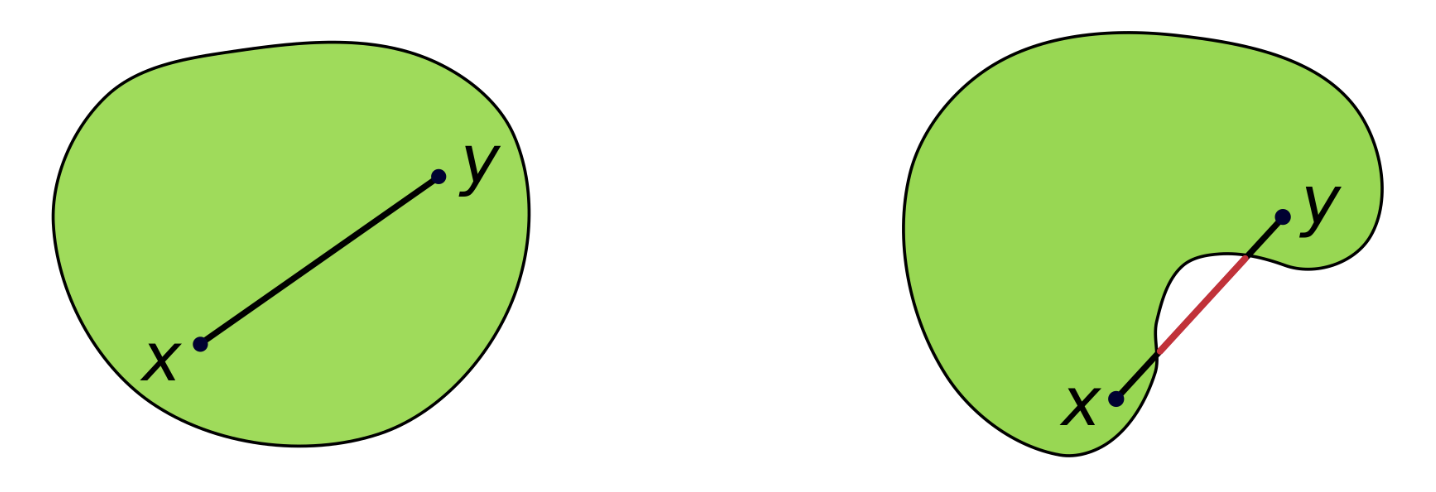
\includegraphics[scale=0.5]{convex.png}
\end{center}
\begin{definition} A set $C \subseteq \R^n$ is \textbf{convex} if for any two points $x, y \in C$, the line segment between $x$ and $y$ is contained in $C$.  In other words, for $x, y \in C$, $\lambda \in [0, 1]$
$$\lambda x + (1 - \lambda) y \in C.$$
\end{definition}
\begin{definition}
Given a subset $S$ of the plane, the convex hull (denoted $\text{conv(S)}$) is the smallest convex set containing $S$.
\begin{center}
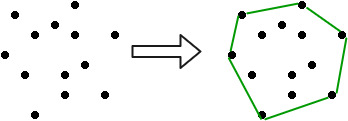
\includegraphics[scale=0.7]{convHull.jpg}
\end{center}
\end{definition}
\pagebreak
\section{Examples}
\begin{prob}[Happy-Ending Problem] Suppose we have five points in the plane with no three collinear.  Show that we can find four points whose convex hull is a quadrilateral.
\end{prob}
\begin{proof}
Take the convex hull of the five points.  If it is a quadrilateral or pentagon, we are done(choose any 4 points in the latter case).  Suppose the convex hull is a triangle.  Label the points with $A$ through $E$ and without loss of generality, let the points $A$, $B$, $C$ form the triangle and $D$, $E$, be the points inside the hull.

Extend the line $DE$.  Note that two points must lie on one side of the line - if not then we have three collinear points.  It is easy to show that these four points form a convex quadrilateral. 
\end{proof}
\begin{prob} There are $n > 3$ coplanar points, no three collinear and every four of them are the vertices of a convex quadrilateral.  Prove that the $n$ points are the vertices of a convex $n$-sided polygon.
\end{prob}
\begin{proof}
Suppose that some point $P$ is inside the convex hull of the $n$ points.  Let $Q$ be some vertex of the convex hull.  The diagonals from $Q$ to the other vertices divide the convex hull into triangles and since no three points are collinear, $P$ must lie inside some triangle $\triangle QRS$.  But this is a contradiction since $P, Q, R, S$ do not form a convex quadrilateral.
\end{proof}

\begin{prob}[1985 IMO Longlist] Let $A, B$ be finite disjoint sets of points in the plane such that any three distinct points in $A \cup B$ are not collinear.  Assume that at least one of the sets $A, B$ contains at least five points.  Show that there exists a triangle all of whose vertices are contained in $A$ or in $B$ that does not contain in its interior any point from the other set.
\end{prob}
\begin{proof}
Suppose $A$ has at least five points.  Take $A_1A_2$ on the boundary of the convex hull of $A$.  For any other $A_i \in A$, define $\theta_i = \angle A_1A_2A_i$.  Without loss of generality, $\theta_3 < \theta_4 < \dots < 180^\circ$.  It follows that $\text{conv}(\{A_1, A_2, A_3, A_4, A_5\})$ contains no other points of $A$.
\end{proof}
\pagebreak
\section{Problems}
\begin{prob}[Putnam 2001 B6] Assume that $(a_n)_{n \ge 1}$ is an increasing sequence of positive real numbers such that $\lim \frac{a_n}{n} = 0$.  Must there exist infinitely many positive integers $n$ such that 
$$a_{n-i} + a_{n+i} < 2a_n$$
for $i = 1, \dots, n-1$?
\end{prob}
\begin{proof}
We claim that such a subsequence exists.  Let $A$ be the convex hull of the points $(n, a_n)$ for $n \ge 0$.  We show that there are infinitely many points on the boundary of $A$ which satisfy the condition.  

If $(n, a_n)$ is on the boundary of $A$, then there is a line through $(n, a_n)$ with all other points of $A$ below the line.  In other words, there exists a slope $m > 0$ such that $$a_k < a_n + m(k-n)$$
for all $k \ge 1$.  

For $n = 1$, since $\frac{a_k}{k} \to 0$, it follows that $$\frac{a_k-a_1}{k-1} \to 0,$$
so the sequence $\{(a_k - a_1)/(k-1)\}$ is bounded.  If we let $m$ be the upper bound, then $$a_k \le a_1 + m(k-1).$$

Now, suppose there is some $n$ satisfying the condition.  Since $\frac{a_k}{k} \to 0$ it follows that 
$$\frac{a_k-a_n}{k-n} \to 0,$$
and $\{(a_k - a_n)/(k-n)\}$ is bounded, which implies that it has a maximum element.  If we let $k = r$ be the largest value where the maximum is attained, set $m = \frac{a_r - a_n}{r-n}$.  The line through $(r, a_r)$ of slope $m$ lies above $(k, a_k)$ for $k > r$ and passes through or lies above $(k, a_k)$ for $k < r$.  It follows that the condition holds for $n = r$ with $m$ replaced by $m - \epsilon$ for some small $\epsilon>0$.

Hence, there are infinitely points on the boundary of $A$.  For each $n$ on the boundary, there exists $m > 0$ such that for $i = 1, \dots, n-1$, the points $(n-i, a_{n-i})$ and $(n+i, a_{n+i})$ lie below the line through $(n, a_n)$ of slope $m$.  It follows that $a_{n+i} < a_n + mi$ and $a_{n-i} < a_n - m_i$, so $a_{n-i} + a_{n+i} < 2a_n$, as desired.
\end{proof}
\end{document}
